% Provenance (never printed): lycee terminale S SVT "Les climats de la Terre"
% and the 2019 enseignement scientifique ("Le climat de la Terre": forcing,
% feedbacks, the IPCC assessments, scenarios), union; physical science only,
% as the user ruled (2026-10-22). See sources/outline_sources.md. Pilot
% chapter, 2026-10-22. Every figure about the climate system is an IPCC AR6
% WG1 statement (ledger ipcc:*) or computed from a dataset in
% figdata/grade-12/climate_records.py.
\chapter{气候变化：观测、成因与预估}\label{ch:g12:climate-change}

位于太平洋中部的莫纳罗亚火山北坡高处，
一组白色建筑矗立在裸露的熔岩上，
海拔 \qty{3397}{m}。这里高于被下方岛屿污染的那层空气，
远离任何大城市数千千米，空气
的洁净和混合程度大致与整个行星的大气相当。
自 1958 年 3 月起，这里的二氧化碳几乎未曾间断地被测量。
这一记录始于一位化学家的个人项目，如今已成为地球科学中
最著名的曲线。本章解读这条曲线及其他气候记录，
说明空气的变化如何改变地球的\omterm{def:g10:earth-energy-budget:energy-budget}{能量收支}，
讨论科学家如何判定所观测到的变暖由何种原因造成，
并给出未来几十年的\omterm{def:g12:climate-change:scenario}{预估}。
% ledger: noaa:mlo-site, noaa:keeling-1958

\begin{omfigure}
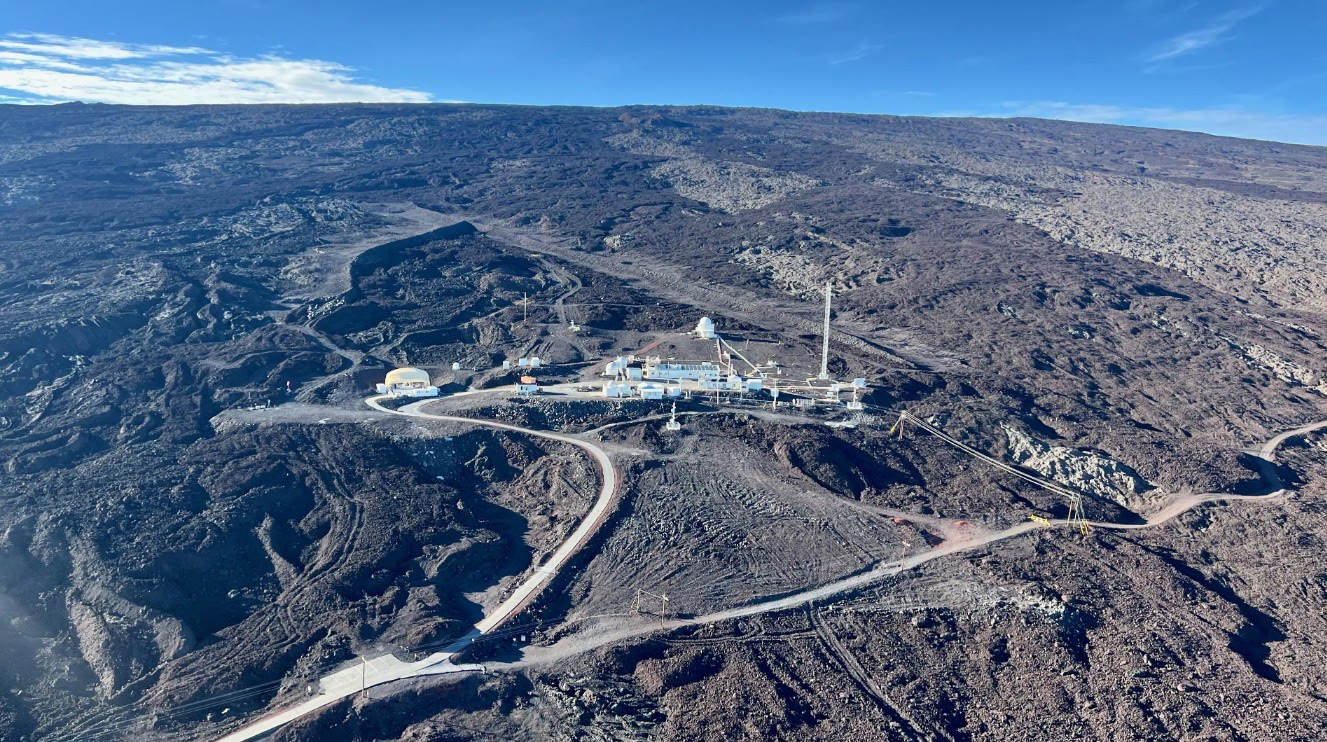
\includegraphics[width=0.78\linewidth]{images/book2/g12-noaa-mauna-loa-observatory.jpg}

{\small 夏威夷莫纳罗亚观测站，位于火山北侧高处的
古老熔岩流上。照片：Brian Vasel, NOAA（公有领域）。}
\end{omfigure}

\begin{recall}
地球以光的形式从太阳接收能量，平均以相同的量
以红外辐射的形式散失到太空；被反射的太阳光比例
即为\omterm{def:g10:earth-energy-budget:albedo}{反照率}（\cref{ch:g10:earth-energy-budget}）。温室气体——水蒸气、
二氧化碳和甲烷——吸收地表
发出的部分红外辐射，并将其中一部分送回地面；这种温室效应使地表
的温度远高于其他情况下的水平（参见化学教材，以及
第 1 册九年级）。\omterm{def:g12:past-climates:ice-core}{冰芯}保存着古代空气的气泡，并记录了
过去 800\,000 年的\omterm{def:g12:past-climates:glacial-cycle}{冰期旋回}（见\cref{ch:g12:past-climates}）。
\end{recall}

\section{各项记录}

\begin{omfigure}
\begin{tikzpicture}
\begin{axis}[omrecord, width=0.92\linewidth, height=6.2cm, xmin=1957, xmax=2028,
  ymin=305, ymax=440, xlabel={年}, ylabel={二氧化碳（ppm）},
  xtick={1960,1970,...,2020}, /pgf/number format/1000 sep={}]
\addplot[omDef!85!black, line width=0.5pt] table[x=decimal_year, y=co2_ppm] {figdata/out/grade-12-climate_records-co2.dat};
\addplot[only marks, mark=*, mark size=0.9pt, omThm!85!black] table[x=year, y=co2_ppm] {figdata/out/grade-12-climate_records-co2annual.dat};
\end{axis}
\end{tikzpicture}

{\small 夏威夷莫纳罗亚站空气中二氧化碳含量：月均值
（折线）与年均值（圆点），以干空气中的百万分之一（ppm）计。
数据来源：NOAA Global Monitoring Laboratory 与 Scripps Institution of
Oceanography。}
\end{omfigure}

\begin{proposition}[二氧化碳记录]\label{prop:g12:climate-change:co2}
% ledger: data:co2-mlo (all numbers computed in figdata/grade-12/climate_records.py)
在莫纳罗亚，二氧化碳的年均浓度由
1959 年的 \qty{316.0}{ppm} 升至 2025 年的 \qty{427.4}{ppm}，并且上升
速度越来越快：1960 年代浓度每年约增加
\qty{0.9}{ppm}，2015 年至 2025 年间则每年约增加 \qty{2.6}{ppm}。每年
浓度还会波动约 \qty{7}{ppm}：最高在
5 月，最低在 9 月。
\end{proposition}

\begin{remark}[曲线为何呈锯齿状]\label{rem:g12:climate-change:teeth}
年内起伏反映的是北半球植被的“呼吸”，
北半球聚集了大部分陆生植物。春夏季，植物通过
光合作用吸收的二氧化碳多于它们和土壤所释放的量；
秋冬季，分解和呼吸作用占上风。逐年的上升
则是另一回事：来自化石燃料和被砍伐森林的碳
正在大气中不断积累。
\end{remark}

\begin{proposition}[高于至少 200 万年以来的水平]\label{prop:g12:climate-change:icecore}
% ledger: data:co2-bereiter (173.7 and 298.6 ppm computed), ipcc:co2-2myr (high confidence)
过去 800\,000 年间，南极冰层中的气泡记录了
二氧化碳浓度在最寒冷的\omterm{def:g12:past-climates:glacial-cycle}{冰期}约为 \qty{174}{ppm}，
在最温暖的\omterm{def:g12:past-climates:glacial-cycle}{间冰期}约为 \qty{299}{ppm}。当今的数值
比其中最高值高出 \qty{100}{ppm} 以上。评估报告指出，
2019 年的浓度高于
至少 200 万年以来的任何时候（\emph{高置信度}）。
\end{proposition}

\begin{omfigure}
\begin{tikzpicture}
\begin{axis}[omrecord, omage, width=0.92\linewidth, height=5.2cm, xmin=0, xmax=810,
  ymin=150, ymax=490, xlabel={1950 年前（千年）},
  ylabel={二氧化碳（ppm）}, xtick={0,100,...,800}]
\addplot[omDef!85!black, line width=0.6pt] table[x=age_kyr, y=co2_ppm] {figdata/out/grade-12-climate_records-icecore.dat};
\draw[omThm, densely dashed, line width=0.8pt] (axis cs:810,427.35) -- (axis cs:0,427.35);
\node[font=\footnotesize, text=omThm!85!black, anchor=south west] at (axis cs:780,433) {2025 年莫纳罗亚年均值};
\end{axis}
\end{tikzpicture}

{\small 南极冰中过去 800\,000 年的二氧化碳含量：\omterm{def:g12:past-climates:glacial-cycle}{冰期
旋回}使其在约 180 至 \qty{300}{ppm} 之间波动。图右端的
细峰代表最年轻的冰，记录了当前上升的开始，
截至 2001 年。数据来源：Bereiter 等（2015），NOAA
Paleoclimatology。}
% the youngest sample of the composite: age -51 yr BP (2001), 368.02 ppm (data/derived/co2-icecore.csv)
\end{omfigure}

\begin{omfigure}
\begin{tikzpicture}
\begin{axis}[omrecord, width=0.92\linewidth, height=5.6cm, xmin=1878, xmax=2027,
  ymin=-0.6, ymax=1.45, xlabel={年},
  ylabel={温度距平（\unit{\degreeCelsius}）},
  xtick={1880,1900,...,2020}, /pgf/number format/1000 sep={},
  legend style={at={(0.03,0.96)}, anchor=north west, font=\footnotesize, draw=black!30}]
\addplot[omDef!70, line width=0.5pt, mark=*, mark size=0.6pt] table[x=year, y=anomaly] {figdata/out/grade-12-climate_records-temp.dat};
\addlegendentry{年均值}
\addplot[omThm!85!black, line width=1.3pt, unbounded coords=jump] table[x=year, y=mean11] {figdata/out/grade-12-climate_records-temp.dat};
\addlegendentry{11 年平均值}
\end{axis}
\end{tikzpicture}

{\small 全球平均地表温度，以其相对于
1951--1980 年平均值的差值表示。数据：NASA GISS 地表温度分析（GISTEMP v4）。}
\end{omfigure}

\begin{proposition}[观测到的全球变暖]\label{prop:g12:climate-change:warming}
% ledger: ipcc:gsat-2011-2020, ipcc:decades
自 1850 年以来，最近四个十年中的每一个都比
它之前的任何一个十年更暖。2011--2020 年的全球地表温度
比 1850--1900 年高 \qty{1.09}{\degreeCelsius}（很可能介于 0.95 与
\qty{1.20}{\degreeCelsius} 之间），陆地增温
（\qty{1.59}{\degreeCelsius}）大于海洋（\qty{0.88}{\degreeCelsius}）。
\end{proposition}

\begin{proposition}[海平面上升越来越快]\label{prop:g12:climate-change:sea}
% ledger: ipcc:sea-level-obs, data:gmsl-lsa (3.2 mm/yr trend computed)
1901 至 2018 年间，全球平均海平面上升约 \qty{0.20}{m}。
1901 至 1971 年间，上升速率约为每年 \qty{1.3}{mm}，
1971 至 2006 年间为每年 \qty{1.9}{mm}，2006 至
2018 年间为每年 \qty{3.7}{mm}（\emph{高置信度}）。自 1993 年起，卫星测量
海面高度，得出平均上升速率为每年 \qty{3.2}{mm}，
时段为 1993--2025 年。海水上升，是因为变暖的海洋膨胀，也因为
冰川和冰盖向海洋输入融冰。
\end{proposition}

\begin{omfigure}
\begin{tikzpicture}
\begin{axis}[omrecord, width=0.86\linewidth, height=5cm, xmin=1992, xmax=2026,
  ymin=-35, ymax=95, xlabel={年}, ylabel={海平面高度（mm）},
  /pgf/number format/1000 sep={}, xtick={1995,2000,...,2025}]
\addplot[omDef!85!black, line width=0.5pt] table[x=decimal_year, y=gmsl_mm] {figdata/out/grade-12-climate_records-sea.dat};
\end{axis}
\end{tikzpicture}

{\small 从太空测得的全球平均海平面，约每十天一次
（已去除季节信号），相对于任意零点。测高数据由
NOAA 卫星测高实验室提供。}
\end{omfigure}

\begin{dated}{2025}
% ledger: data:co2-mlo, data:gistemp (values read from the datasets as fetched 2026-10-22)
2025 年，莫纳罗亚站的年均二氧化碳浓度为
\qty{427.35}{ppm}。在 NASA 的温度记录中，迄今最暖的一年为
2024 年，比 1951--1980 年平均值高 \qty{1.28}{\degreeCelsius}。
\end{dated}

\section{辐射强迫}

\begin{definition}[辐射强迫]\label{def:g12:climate-change:forcing}
气候系统中某一变化的\emph{辐射强迫}\index{辐射强迫}
（如温室气体增多、气溶胶颗粒增多、太阳变亮），
是指在地表温度来得及响应之前，该变化引起的、
在大气层顶进入气候系统的净能量流的改变量。
它以瓦特每平方米计量，
（\unit{W/m^2}），以地球表面计。
正辐射强迫使行星获得能量而变暖，负辐射强迫使其失去能量而变冷。
\end{definition}

\begin{remark}[有效辐射强迫]\label{rem:g12:climate-change:effective}
评估报告采用的是\emph{有效}\omterm{def:g12:climate-change:forcing}{辐射强迫}，它还计入大气的快速调整，
例如云的变化，
这些调整发生在地表变暖之前。本章中的所有强迫
均为有效\omterm{def:g12:climate-change:forcing}{辐射强迫}。
\end{remark}

\begin{proposition}[1750 年以来的辐射强迫]\label{prop:g12:climate-change:forcing}
% ledger: ipcc:erf-total, ipcc:erf-agents
以 1750 年为基准，2019 年人类活动产生的\omterm{def:g12:climate-change:forcing}{辐射强迫}总量为
\qty{2.72}{W/m^2}（很可能介于 1.96 与
\qty{3.48}{W/m^2} 之间）。温室气体贡献正强迫，其中以
二氧化碳最为突出（\qty{2.16}{W/m^2}）；气溶胶颗粒能反射阳光并使云层变亮，
贡献负强迫（合计约
\qty{-1.06}{W/m^2}）。太阳亮度在同一时期的变化
仅贡献 \qty{0.01}{W/m^2}。
\end{proposition}

\begin{omfigure}
% ledger: ipcc:erf-agents, ipcc:erf-total (central values and 5-95 % ranges of AR6 Table 7.8)
\begin{tikzpicture}
\begin{axis}[xbar, width=0.8\linewidth, height=7.2cm, xmin=-1.8, xmax=3.7,
  ytick={1,...,10}, yticklabels={总计（人为）,太阳,土地利用,
  气溶胶–云,气溶胶–辐射,臭氧,卤代气体,氧化亚氮,
  甲烷,二氧化碳}, y tick label style={font=\small},
  tick label style={font=\small}, xlabel={有效辐射强迫，1750--2019 年（\unit{W/m^2}）},
  label style={font=\small}, bar width=6pt, bar shift=0pt, axis x line=bottom, axis y line=left,
  axis line style={-}, enlarge y limits=0.07, xmajorgrids,
  grid style={gray!22, line width=0.3pt}, extra x ticks={0},
  extra x tick style={grid style={black!60, line width=0.5pt}}]
\addplot[fill=omThm!55, draw=omThm!80!black, error bars/.cd, x dir=both, x explicit,
  error bar style={black!70}] coordinates {
  (2.16,10) += (0.25,0) -= (0.26,0)
  (0.54,9) += (0.11,0) -= (0.11,0)
  (0.21,8) += (0.03,0) -= (0.03,0)
  (0.41,7) += (0.08,0) -= (0.08,0)
  (0.47,6) += (0.24,0) -= (0.23,0)
  (2.72,1) += (0.76,0) -= (0.76,0)
  (0.01,2) += (0.07,0) -= (0.07,0)};
\addplot[fill=omDef!55, draw=omDef!80!black, error bars/.cd, x dir=both, x explicit,
  error bar style={black!70}] coordinates {
  (-0.22,5) += (0.26,0) -= (0.25,0)
  (-0.84,4) += (0.59,0) -= (0.61,0)
  (-0.20,3) += (0.10,0) -= (0.10,0)};
\end{axis}
\end{tikzpicture}

{\small 1750 至 2019 年间主要的有效\omterm{def:g12:climate-change:forcing}{辐射强迫}及其
很可能范围（误差线）。数值来源：IPCC Sixth Assessment Report，Working
Group~I，表 7.8。}
\end{omfigure}

\begin{proposition}[二氧化碳：每次加倍增加的强迫相同]\label{prop:g12:climate-change:log}
% ledger: ipcc:erf-2xco2, ipcc:log-co2
近似地，二氧化碳的强迫随其浓度的
\emph{对数}而增长：每次加倍增加的强迫相同，
$F_{2\times} = \qty{3.93}{W/m^2}$ 为自 1750 年
浓度 $C_0 = \qty{278}{ppm}$ 出发的一次加倍所对应的强迫。浓度 $C$ 对应的强迫则为
\[
  F = F_{2\times}\,\frac{\ln (C/C_0)}{\ln 2}.
\]
\end{proposition}

\begin{example}[依据评估结果检验该规律]\label{ex:g12:climate-change:check}
% ledger: ipcc:erf-2xco2, ipcc:erf-agents
2019 年的浓度为 \qty{410}{ppm}。由规律可得
$F = 3.93 \times \ln(410/278)/\ln 2 = 3.93 \times 0.561 \approx
\qty{2.20}{W/m^2}$，与评估中二氧化碳在 1750--2019 年间
所给出的 \qty{2.16}{W/m^2} 相差不到 2\,\%。
\end{example}

\begin{proposition}[多余的能量去向何方]\label{prop:g12:climate-change:heating}
% ledger: ipcc:heating
由于强迫为正，气候系统获得能量：2006--2018 年间平均约为
\qty{0.79}{W/m^2}，高于 1971--2006 年间的 \qty{0.50}{W/m^2}
（\emph{高度可信}）。海洋吸收了这部分能量的 91\,\%；
陆地吸收 5\,\%，融化的冰吸收 3\,\%，大气仅吸收 1\,\%。
\end{proposition}

\section{反馈与气候敏感度}

地表变暖时，它向太空辐射的能量增多，这倾向于使行星
恢复平衡。变暖还会改变其他事物——
空气中的水汽、地面的雪和冰、
云——这些变化又反过来改变\omterm{def:g10:earth-energy-budget:energy-budget}{能量收支}。

\begin{definition}[气候反馈]\label{def:g12:climate-change:feedback}
\emph{气候反馈}\index{气候反馈}是气候系统中的一种变化，
由温度变化引起，它改变\omterm{def:g10:earth-energy-budget:energy-budget}{能量收支}，进而改变温度变化本身。
\emph{正反馈}放大最初的变化；
\emph{负反馈}则抑制它。
\end{definition}

\begin{example}[三种反馈]\label{ex:g12:climate-change:three}
\begin{itemize}
  \item \textbf{水汽（正反馈）。} 气温升高时，空气能容纳更多水汽，
        水汽是一种温室气体，会加剧变暖。
  \item \textbf{雪和冰（正反馈）。} 雪和冰反射太阳光；
        它们融化后，下面较暗的陆地和海面会吸收更多太阳辐射，
        变暖随之加剧。
  \item \textbf{向太空辐射（负反馈）。} 地表和大气变暖后，
        向太空辐射的红外线增多。这一基本响应
        最终总会占上风：正因如此，气候才会稳定在一个新的、
        更暖的平衡上，而不会无限制地变暖。
\end{itemize}
\end{example}

\begin{omfigure}
\begin{tikzpicture}[font=\small, >={Stealth[length=2.4mm]},
  box/.style={draw=black!60, rounded corners=2pt, fill=white, align=center,
  inner sep=3pt, text width=3cm}]
  \node[box, fill=omThm!12] (w) at (0,0) {地表变暖};
  \node[box] (v) at (3.6,1.3) {空气中水汽增多};
  \node[box] (g) at (3.6,-1.3) {增强的 \\温室效应};
  \draw[->, omThm!85!black, thick] (w) to[bend left=18] (v);
  \draw[->, omThm!85!black, thick] (v) -- (g);
  \draw[->, omThm!85!black, thick] (g) to[bend left=18] (w);
  \node[font=\footnotesize, text=omThm!85!black] at (2.0,0) {$+$};
  \node[box] (s) at (-3.6,1.3) {冰雪融化};
  \node[box] (a) at (-3.6,-1.3) {反照率降低：吸收更多太阳光};
  \draw[->, omThm!85!black, thick] (w) to[bend right=18] (s);
  \draw[->, omThm!85!black, thick] (s) -- (a);
  \draw[->, omThm!85!black, thick] (a) to[bend right=18] (w);
  \node[font=\footnotesize, text=omThm!85!black] at (-2.0,0) {$+$};
  \node[box] (r) at (0,-2.9) {向太空辐射更多红外线};
  \draw[->, omDef!85!black, thick] ([xshift=-0.35cm]w.south) -- ([xshift=-0.35cm]r.north);
  \draw[->, omDef!85!black, thick] ([xshift=0.35cm]r.north) -- ([xshift=0.35cm]w.south);
  \node[font=\footnotesize, text=omDef!85!black] at (0.62,-1.45) {$-$};
\end{tikzpicture}

{\small 两条正反馈回路（红色）放大变暖；变暖行星向外辐射的
额外红外线（蓝色）是一种负反馈，
它限制变暖。}
\end{omfigure}

\begin{proposition}[平衡时的变暖]\label{prop:g12:climate-change:equilibrium}
% ledger: ipcc:feedbacks
气候达到新的平衡后，变暖量 $\Delta T$ 由
恒定强迫 $F$ 引起，为
\[
  \Delta T = \frac{F}{\lambda},
\]
其中 $\lambda$ 为\emph{\omterm{def:g12:climate-change:feedback}{气候反馈}参数}，表示
温度每升高一度，行星向太空额外损失的能量。评估将
向太空的辐射（$\qty{3.22}{W.m^{-2}.\degreeCelsius^{-1}}$）
与水汽和温度剖面的正反馈
（$1.30$）、地表\omterm{def:g10:earth-energy-budget:albedo}{反照率}的正反馈（$0.35$）以及云的正反馈（$0.42$，
单位相同）合并为 $\lambda \approx \qty{1.16}{W.m^{-2}.\degreeCelsius^{-1}}$。
\end{proposition}

\begin{proof}[部分证明]
新的平衡状态下，气候系统向太空损失的能量
再次与获得的能量相等，因此变暖导致的额外损失 $\lambda\,\Delta T$ 必须
抵消强迫：$\lambda\,\Delta T = F$。额外损失与
$\Delta T$ 成正比是一种近似，适用于几度的变暖，
此处在本阶段不加证明地承认。
\end{proof}

\begin{definition}[平衡气候敏感度]\label{def:g12:climate-change:ecs}
\emph{平衡气候敏感度}\index{平衡气候敏感度}是指，
在二氧化碳浓度从 1750 年水平加倍后，
达到新的平衡时地球表面的变暖幅度。
\end{definition}

\begin{proposition}[气候有多敏感？]\label{prop:g12:climate-change:ecs}
% ledger: ipcc:ecs
综合各方面的证据——反馈的物理机制、
观测到的变暖、过去的气候——评估给出\omterm{def:g12:climate-change:ecs}{平衡气候敏感度}的
最佳估计值为 \qty{3}{\degreeCelsius}，可能介于
2.5 至 \qty{4}{\degreeCelsius} 之间（\emph{高度可信}），
并且很可能介于 2 至 \qty{5}{\degreeCelsius} 之间。
\end{proposition}

\section{谁应负责？}

\begin{method}[解读评估中的表述]\label{met:g12:climate-change:language}
% ledger: ipcc:likelihood
气候科学的国际评估以固定的词汇对每项结论进行分级，
这些词汇以斜体印出：
\begin{itemize}
  \item \emph{可能性}，即某一结果发生的概率：
        \emph{几乎确定} 99--100\,\%，\emph{极可能}
        95--100\,\%，\emph{很可能} 90--100\,\%，\emph{可能}
        66--100\,\%，\emph{大致同样可能} 33--66\,\%，
        \emph{不太可能} 0--33\,\%，\emph{很不可能} 0--10\,\%；
  \item \emph{可信度}，即一项结论背后证据的强度与
        共识的一致程度：很低、低、中、高、很高。
\end{itemize}
形如 $[x \text{ 至 } y]$ 的区间是很可能区间，即真值落在其中的
概率为 90\,\%。读懂一条表述时，应确定
所讨论的量、其最佳估计值、取值范围，以及所附的可能性或
可信度。
\end{method}

\begin{definition}[归因]\label{def:g12:climate-change:attribution}
\emph{归因}\index{归因}是对一项观测到的变化，评估其中各个可能原因分别
所占的比例，并给出该结果的
可能性。
\end{definition}

\begin{proposition}[人类影响]\label{prop:g12:climate-change:attribution}
% ledger: ipcc:unequivocal, ipcc:attribution, ipcc:observed-2010-2019
毫无疑义的是，人类影响已使大气、海洋
和陆地变暖。1850--1900 年与 2010--2019 年相比，全球地表升温约
\qty{1.06}{\degreeCelsius}。人类活动造成的升温为
\qty{0.8}{\degreeCelsius} 至 \qty{1.3}{\degreeCelsius}（可能区间），最佳
估计值为 \qty{1.07}{\degreeCelsius}：充分混合的温室气体很可能
使地表升温 1.0 至 \qty{2.0}{\degreeCelsius}，其他人为影响
主要是气溶胶，很可能使其降温 0 至
\qty{0.8}{\degreeCelsius}。太阳和火山的影响仅为 $-0.1$
至 $+\qty{0.1}{\degreeCelsius}$，气候的自然波动为
$-0.2$ 至 $+\qty{0.2}{\degreeCelsius}$。
\end{proposition}

\begin{omfigure}
% ledger: ipcc:attribution, ipcc:observed-2010-2019
\begin{tikzpicture}
\begin{axis}[width=0.7\linewidth, height=5.6cm, xmin=-1, xmax=2.2, ymin=0.4, ymax=6.6,
  ytick={1,...,6}, yticklabels={自然变率,太阳和火山,
  气溶胶及其他人为因素,温室气体,所有人为影响,观测值},
  y tick label style={font=\small}, tick label style={font=\small},
  xlabel={1850--1900 至 2010--2019 年间的升温贡献 (\unit{\degreeCelsius})},
  label style={font=\small}, axis x line=bottom, axis y line=left, axis line style={-},
  xmajorgrids, grid style={gray!22, line width=0.3pt}, extra x ticks={0},
  extra x tick style={grid style={black!60, line width=0.5pt}}]
\draw[black!70, line width=5pt] (axis cs:0.88,6) -- (axis cs:1.21,6);
\fill (axis cs:1.06,6) circle (2.4pt);
\draw[omThm!80, line width=5pt] (axis cs:0.8,5) -- (axis cs:1.3,5);
\fill (axis cs:1.07,5) circle (2.4pt);
\draw[omThm!55, line width=5pt] (axis cs:1.0,4) -- (axis cs:2.0,4);
\draw[omDef!60, line width=5pt] (axis cs:-0.8,3) -- (axis cs:0,3);
\draw[gray!70, line width=5pt] (axis cs:-0.1,2) -- (axis cs:0.1,2);
\draw[gray!45, line width=5pt] (axis cs:-0.2,1) -- (axis cs:0.2,1);
\end{axis}
\end{tikzpicture}

{\small 观测升温的成因：各项贡献的可能区间，
有评估给出时标出最佳估计值（圆点）；对观测升温，
观测升温的很可能区间。数值引自 IPCC Sixth Assessment
Report, Working Group~I, Summary for Policymakers, A.1.3。}
\end{omfigure}

\section{情景与预估}

\begin{definition}[情景与预估]\label{def:g12:climate-change:scenario}
\emph{排放情景}\index{排放情景}是一种自洽的
描述，说明温室气体和气溶胶的排放在
未来可能如何演变。\emph{预估}\index{预估（气候）}是模式针对给定情景
计算出的气候响应。预估不是预报：
它说明\emph{若}该情景成真，将会发生什么。
\end{definition}

\begin{proposition}[预估升温与海平面上升]\label{prop:g12:climate-change:projections}
% ledger: ipcc:proj-temp, ipcc:proj-sea, ipcc:3myr
评估采用五种主要情景，排放从很低（SSP1-1.9）
到很高（SSP5-8.5）。与 1850--1900 年相比，2081--2100 年
的升温\omterm{def:g12:climate-change:scenario}{预估}如下（最佳估计值与很可能区间，单位
\unit{\degreeCelsius}），以及到 2100 年相对 1995--2014 年的
全球平均海平面可能上升幅度。在各情景下，海平面在本世纪内都
持续上升（\emph{几乎确定}）。全球地表最近一次
维持高于 1850--1900 年 \qty{2.5}{\degreeCelsius} 或以上，是在
三百多万年前（\emph{中等可信度}）。

\begin{center}
\small
\begin{tabular}{lccc}
\hline
情景 & 排放 & 2081--2100 年升温 (\unit{\degreeCelsius}) & 到 2100 年海平面上升 (m) \\
\hline
SSP1-1.9 & 很低 & 1.4 （1.0 至 1.8） & 0.28 至 0.55 \\
SSP1-2.6 & 低 & 1.8 （1.3 至 2.4） & 0.32 至 0.62 \\
SSP2-4.5 & 中等 & 2.7 （2.1 至 3.5） & 0.44 至 0.76 \\
SSP3-7.0 & 高 & 3.6 （2.8 至 4.6） &——\\
SSP5-8.5 & 很高 & 4.4 （3.3 至 5.7） & 0.63 至 1.01 \\
\hline
\end{tabular}
\end{center}
\end{proposition}

\begin{omfigure}
% ledger: ipcc:proj-temp
\begin{tikzpicture}
\begin{axis}[width=0.8\linewidth, height=5.2cm, xmin=0.4, xmax=5.6, ymin=0, ymax=6.2,
  xtick={1,...,5}, xticklabels={SSP1-1.9, SSP1-2.6, SSP2-4.5, SSP3-7.0, SSP5-8.5},
  x tick label style={font=\small}, tick label style={font=\small},
  ylabel={2081--2100 年升温 (\unit{\degreeCelsius})}, label style={font=\small},
  axis x line=bottom, axis y line=left, axis line style={-}, ymajorgrids,
  grid style={gray!22, line width=0.3pt}]
\draw[omThm!60, line width=9pt] (axis cs:1,1.0) -- (axis cs:1,1.8);
\draw[black, line width=1.2pt] (axis cs:0.83,1.4) -- (axis cs:1.17,1.4);
\draw[omThm!60, line width=9pt] (axis cs:2,1.3) -- (axis cs:2,2.4);
\draw[black, line width=1.2pt] (axis cs:1.83,1.8) -- (axis cs:2.17,1.8);
\draw[omThm!60, line width=9pt] (axis cs:3,2.1) -- (axis cs:3,3.5);
\draw[black, line width=1.2pt] (axis cs:2.83,2.7) -- (axis cs:3.17,2.7);
\draw[omThm!60, line width=9pt] (axis cs:4,2.8) -- (axis cs:4,4.6);
\draw[black, line width=1.2pt] (axis cs:3.83,3.6) -- (axis cs:4.17,3.6);
\draw[omThm!60, line width=9pt] (axis cs:5,3.3) -- (axis cs:5,5.7);
\draw[black, line width=1.2pt] (axis cs:4.83,4.4) -- (axis cs:5.17,4.4);
\end{axis}
\end{tikzpicture}

{\small 五种情景下本世纪末的\omterm{def:g12:climate-change:scenario}{预估}升温：
很可能范围（柱）与最佳估计（黑线）。数值来源：IPCC Sixth
Assessment Report，Working Group~I，表 SPM.1。}
\end{omfigure}

\begin{remark}[本章未说明的内容]\label{rem:g12:climate-change:science}
世界将遵循哪种情景，取决于未来的排放，也就是
取决于那些不属于物理问题的决策。物理科学说明的
是气候对每一种情景的响应；在它们之间作出选择，属于
社会的事务，其代价与收益则由其他学科研究。
\end{remark}

\begin{history}[一条曲线，起初是一位化学家的项目]
% ledger: noaa:keeling-1958
1958 年 3 月，化学家查尔斯·大卫·基林就职于斯克里普斯
海洋研究所，开始在莫纳罗亚测量空气中的二氧化碳，
所用仪器的精度足以测出不足
百万分之一的变化。数年之内，他的记录既显示了植被每年的呼吸
作用，也显示出稳定的上升。此后的测量由斯克里普斯研究所
与美国国家海洋和大气管理局继续进行，
是大气成分最长的直接记录。
\begin{center}
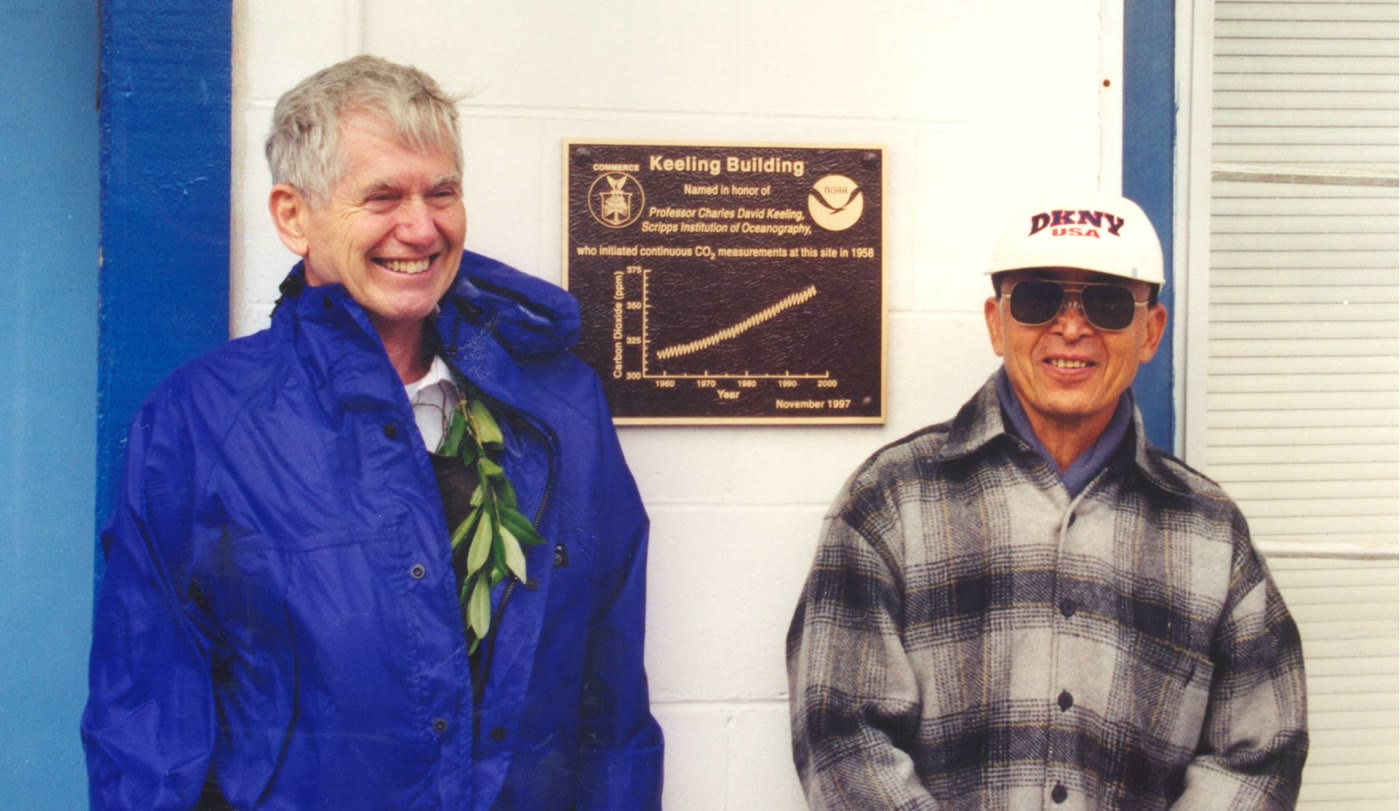
\includegraphics[width=0.62\linewidth]{images/book2/g12-noaa-keeling-chin-1997.jpg}

{\small 查尔斯·大卫·基林（左）与约翰·钦在莫纳罗亚
天文台，1997 年，站在一块以基林命名某座建筑的铭牌旁。
照片：John Miller，NOAA（公有领域）。}
\end{center}
\end{history}

\section{练习}

\begin{exercise}[$\star$]\label{exo:g12:climate-change:1}
气候系统变化的\omterm{def:g12:climate-change:forcing}{辐射强迫}是什么？它以哪种
单位计量，其正负号表示什么含义？
\end{exercise}

\begin{exercise}[$\star$]\label{exo:g12:climate-change:2}
一年中，莫纳罗亚的二氧化碳浓度在哪个月最高，
在哪个月最低？请说明其年度变化。
\end{exercise}

\begin{exercise}[$\star$]\label{exo:g12:climate-change:3}
在评估报告的用语中，\emph{很
可能}对应的概率是多少？\emph{可能}呢？写作
$[0.95 \text{ 至 } 1.20]$ 的范围表示什么？
\end{exercise}

\begin{exercise}[$\star$]\label{exo:g12:climate-change:4}
在近几十年气候系统所获得的额外能量中，
有多大份额进入了海洋？这为何能解释海平面
在没有冰融化时仍会上升？
\end{exercise}

\begin{exercise}[$\star$]\label{exo:g12:climate-change:5}
请给出两个正\omterm{def:g12:climate-change:feedback}{气候反馈}，以及限制变暖的
负反馈，并各用一句话加以解释。
\end{exercise}

\begin{exercise}[$\star\star$]\label{exo:g12:climate-change:6}
莫纳罗亚二氧化碳的年平均浓度在 1959 年为
\qty{315.98}{ppm}，2025 年为 \qty{427.35}{ppm}。增加了多少 ppm，
增幅为百分之几？整个时期内，平均每年的
增长量是多少？
\end{exercise}

\begin{exercise}[$\star\star$]\label{exo:g12:climate-change:7}
利用本章的对数定律，取 $F_{2\times} =
\qty{3.93}{W/m^2}$ 与 $C_0 = \qty{278}{ppm}$，计算二氧化碳在
\qty{427.35}{ppm}（2025 年年平均值）时的\omterm{def:g12:climate-change:forcing}{辐射强迫}。
\end{exercise}

\begin{exercise}[$\star\star$]\label{exo:g12:climate-change:8}
按 2006--2018 年的速率，即 \qty{3.7}{mm} 每年，
30 年内海平面将上升多少？这一速率是
1901--1971 年（\qty{1.3}{mm} 每年）的多少倍？
\end{exercise}

\begin{exercise}[$\star\star$]\label{exo:g12:climate-change:9}
利用 $\Delta T = F/\lambda$，取 $\lambda = \qty{1.16}{W.m^{-2}.\degreeCelsius^{-1}}$，
计算 2019 年人为总\omterm{def:g12:climate-change:forcing}{辐射强迫}
\qty{2.72}{W/m^2} 所产生的平衡升温。观测到的人为增温仅
约 \qty{1.07}{\degreeCelsius}。请给出两者差异的主要原因。
\end{exercise}

\begin{exercise}[$\star\star$]\label{exo:g12:climate-change:10}
太阳与火山活动使全球温度在 1850--1900 年与
2010--2019 年之间变化了 $-0.1$ 至 $+\qty{0.1}{\degreeCelsius}$，而观测到的
增温约为 \qty{1.06}{\degreeCelsius}。由此能得出什么结论？还必须排除哪一种
其他自然原因，评估报告对此
有何说明？
\end{exercise}

\begin{exercise}[$\star\star$]\label{exo:g12:climate-change:11}
利用\omterm{def:g12:climate-change:scenario}{预估}表，2081--2100 年的增温在哪些情景下很可能
保持在 \qty{2}{\degreeCelsius} 以下？在哪些情景下很可能
超过 \qty{2}{\degreeCelsius}？
\end{exercise}

\begin{exercise}[$\star\star\star$]\label{exo:g12:climate-change:12}
气溶胶产生的\omterm{def:g12:climate-change:forcing}{辐射强迫}约为 $-0.22$ 与 $\qty{-0.84}{W/m^2}$
（经由日照与云），若将所有气溶胶从
大气中移除，其余保持 2019 年的状态，则人为总\omterm{def:g12:climate-change:forcing}{辐射强迫}
将变为多少？平衡升温将增加多少（取
$\lambda = \qty{1.16}{W.m^{-2}.\degreeCelsius^{-1}}$）？
\end{exercise}

\begin{exercise}[$\star\star\star$]\label{exo:g12:climate-change:13}
试由对数定律证明，从 \qty{278}{ppm} 增至
\qty{556}{ppm}，以及从 \qty{556}{ppm} 增至 \qty{1112}{ppm}，
两段所增加的\omterm{def:g12:climate-change:forcing}{辐射强迫}相同。\qty{1112}{ppm} 时的总\omterm{def:g12:climate-change:forcing}{辐射强迫}是多少？
\end{exercise}

\begin{exercise}[$\star\star\star$]\label{exo:g12:climate-change:14}
对对数定律关于 $C$ 求导。多增加 1 ppm 的二氧化碳，
在 \qty{280}{ppm} 时会增加多少\omterm{def:g12:climate-change:forcing}{辐射强迫}，在
\qty{420}{ppm} 时又是多少？请加以评述。
\end{exercise}

\begin{exercise}[$\star\star\star$]\label{exo:g12:climate-change:15}
除向太空的额外辐射外，不考虑其他任何反馈，
$\lambda_0 = \qty{3.22}{W.m^{-2}.\degreeCelsius^{-1}}$。试计算
二氧化碳加倍（$F_{2\times} = \qty{3.93}{W/m^2}$）时的升温，
分别以 $\lambda_0$ 和 $\lambda = \qty{1.16}{W.m^{-2}.\degreeCelsius^{-1}}$ 计算。
反馈将升温放大了多少倍？
\end{exercise}

\section{问题：数字中的基林曲线}

\begin{problem}[{周末问题——从植被的年度
呼吸到二氧化碳浓度达到加倍的年份}]
\label{pb:g12:climate-change:1}
% ledger: data:co2-mlo (annual means 1960 316.91, 1970 325.68, 2015 401.01,
% 2025 427.35; seasonal departures May +3.37, September -3.51, means of
% 2015-2024; all from figdata/grade-12/climate_records.py), noaa:mlo-site,
% ipcc:erf-2xco2, ipcc:ecs, ipcc:feedbacks, ipcc:co2-2myr
一名学生下载了莫纳罗亚站的记录，并用电子表格进行处理。
在 2015--2024 年间，5 月的月均浓度比平滑趋势平均高出
\qty{3.37}{ppm}，在 9 月则比其低 \qty{3.51}{ppm}。
年均浓度在 1960 年为 \qty{316.91}{ppm}，
1970 年为 \qty{325.68}{ppm}，2015 年为 \qty{401.01}{ppm}，2025 年为 \qty{427.35}{ppm}。
1750 年的浓度为 \qty{278}{ppm}。请使用对数定律，
取 $F_{2\times} = \qty{3.93}{W/m^2}$。

\medskip
\noindent\textbf{第一部分——植被的呼吸。}
\begin{enumerate}
  \item 年循环的峰谷振幅是多少？
  \item 解释为什么浓度在 5 月最高、在
        9 月最低。
  \item 南半球大气中的这一循环要弱得多。
        试给出原因。
  \item 这座观测站为何建在太平洋中部的火山上，
        海拔 \qty{3397}{m}？
\end{enumerate}

\medskip
\noindent\textbf{第二部分——趋势。}
\begin{enumerate}[resume]
  \item 计算 1960--1970 年间的年均增长量，单位为 ppm/年。
  \item 计算 2015--2025 年间的年均增长量。
  \item 增长速率提高了多少倍？
  \item 1750 年至
        2025 年间，浓度上升了百分之多少？
  \item \omterm{def:g12:past-climates:ice-core}{冰芯}记录显示，在过去 800\,000 年中，浓度从未超过约
        \qty{300}{ppm}。2025 年的数值比
        这一上限高出多少 ppm？
\end{enumerate}

\medskip
\noindent\textbf{第三部分——\omterm{def:g12:climate-change:forcing}{辐射强迫}。}
\begin{enumerate}[resume]
  \item 计算 2025 年二氧化碳的\omterm{def:g12:climate-change:forcing}{辐射强迫}。
  \item 计算 1960 年的\omterm{def:g12:climate-change:forcing}{辐射强迫}，以及 1960 年至
        2025 年间\omterm{def:g12:climate-change:forcing}{辐射强迫}的增量。
  \item 浓度达到多少时，会使 2025 年的\omterm{def:g12:climate-change:forcing}{辐射强迫}增加 \qty{1}{W/m^2}？
  \item 按 2015--2025 年的增长速率，这需要多少年？
\end{enumerate}

\medskip
\noindent\textbf{第四部分——加倍。}
\begin{enumerate}[resume]
  \item 1750 年浓度加倍后为多少？
        它产生多大的\omterm{def:g12:climate-change:forcing}{辐射强迫}？
  \item 取\omterm{def:g12:climate-change:ecs}{平衡气候敏感度}的最佳估计值，
        它会引起多大的平衡升温？给出可能范围。
  \item \omterm{def:g12:climate-change:ecs}{平衡气候敏感度}为 \qty{3}{\degreeCelsius} 时，反馈参数 $\lambda$ 为多少？
        将其与累加各项反馈
        所得的 \qty{1.16}{W.m^{-2}.\degreeCelsius^{-1}}
        进行比较。
  \item 浓度达到加倍的那一天，
        地表为何达不到这一升温？
  \item 为何仅将今日的增长速率延长所作的计算是一种情景，
        而非评估所作的那种\omterm{def:g12:climate-change:scenario}{预估}？
  \item 若 2015--2025 年的增长速率保持不变，
        1750 年浓度将在哪一年达到加倍？
\end{enumerate}
\end{problem}
